\section{Kenapa kita membutuhkan komputasi parallel?}

Pertumbuhan daya komputasi yang disediakan oleh komputer modern telah menghasilkan masalah komputasi yang semakin kompleks dalam jangka waktu yang relatif singkat. Sampai awal 2000-an, kompleksitas ditangani dengan meningkatkan jumlah transistor serta frekuensi clock dari sistem prosesor tunggal, yang mencapai puncak 3,5-4 GHz. Namun, peningkatan jumlah transistor menyebabkan peningkatan eksponensial dari daya yang dihabiskan oleh prosesor itu sendiri. Pada dasarnya, ada, oleh karena itu, keterbatasan fisik yang mencegah peningkatan lebih lanjut dalam kinerja sistem prosesor tunggal.
\noindent
Untuk alasan ini, dalam beberapa tahun terakhir, produsen mikroprosesor memusatkan perhatian mereka pada sistem multi-core. Ini didasarkan pada inti dari beberapa prosesor fisik yang berbagi memori yang sama, sehingga dengan melewatkan masalah daya yang hilang yang dijelaskan sebelumnya. Dalam beberapa tahun terakhir, sistem quad-core dan octa-core juga telah menjadi standar pada konfigurasi desktop dan laptop normal.
\noindent
Di sisi lain, perubahan signifikan dalam perangkat keras juga menghasilkan evolusi struktur perangkat lunak, yang selalu dirancang untuk dieksekusi secara berurutan pada satu prosesor. Untuk mengambil keuntungan dari sumber daya komputasi yang lebih besar yang tersedia dengan meningkatkan jumlah prosesor, perangkat lunak yang ada harus dirancang ulang dalam bentuk yang sesuai dengan struktur paralel CPU, sehingga dapat memperoleh efisiensi yang lebih besar melalui eksekusi simultan dari unit tunggal dari beberapa bagian dari program yang sama.

\section{Taksonomi Flynn}
Taksonomi Flynn adalah sistem untuk mengklasifikasikan arsitektur komputer. Ini didasarkan pada dua konsep utama:

\begin{enumerate}
	\item Instruction flow: Suatu sistem dengan n CPU memiliki n penghitung program dan, oleh karena itu, n instruksi mengalir. Ini sesuai dengan penghitung program.
	\item Data flow: Program yang menghitung fungsi pada daftar data memiliki aliran data. Program yang menghitung fungsi yang sama pada beberapa daftar data yang berbeda memiliki lebih banyak aliran data. Ini terdiri dari seperangkat operan.
\end{enumerate}

\noindent
Karena instruksi dan aliran data bersifat independen, ada empat kategori mesin paralel: Single Instruction Single Data (SISD), Single Instruction Multiple Data (SIMD), Multiple Instruction Single Data (MISD), and Multiple Instruction Multiple Data (MIMD):

\begin{figure}[H]
	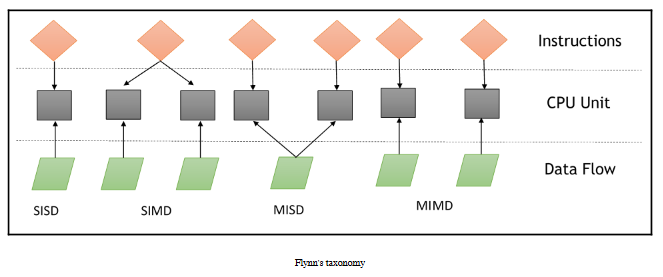
\includegraphics[width=4cm]{figures/kelompok2/chapter1/1.png}
	\centering
	\caption{Flynn.}
\end{figure}

\subsection{Single Instruction Single Data (SISD)}
Sistem komputasi SISD seperti mesin von Neumann, yang merupakan mesin uniprocessor. Seperti yang Anda lihat dalam diagram taksonomi Flynn, ia menjalankan instruksi tunggal yang beroperasi pada aliran data tunggal. Di SISD, instruksi mesin diproses secara berurutan.

\noindent
Dalam siklus clock, CPU menjalankan operasi berikut:

\begin{enumerate}
	\item Fetch: CPU mengambil data dan instruksi dari area memori, yang disebut register.
	\item Decode: CPU menerjemahkan instruksi.
	\item Execute: Instruksi dilakukan pada data. Hasil operasi disimpan dalam register lain.
\end{enumerate}

\noindent
Setelah tahap eksekusi selesai, CPU menetapkan dirinya untuk memulai siklus CPU lain:

\begin{figure}[H]
	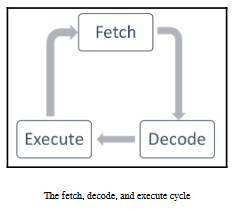
\includegraphics[width=4cm]{figures/kelompok2/chapter1/2.png}
	\centering
	\caption{SISD.}
\end{figure}

\noindent
Algoritma yang berjalan pada komputer jenis ini bersifat berurutan (atau serial) karena tidak mengandung paralelisme. Contoh komputer SISD adalah sistem perangkat keras dengan satu CPU.

\noindent
Elemen utama dari arsitektur ini (yaitu, arsitektur von Neumann) adalah sebagai berikut:

\begin{enumerate}
	\item Central memori unit: Ini digunakan untuk menyimpan instruksi dan data program.
	\item CPU: Ini digunakan untuk mendapatkan instruksi dan / atau data dari unit memori, yang menerjemahkan instruksi dan secara berurutan mengimplementasikannya.
	\item The I/O system: Ini mengacu pada data input dan output dari program.
\end{enumerate}

\noindent
Komputer prosesor tunggal konvensional diklasifikasikan sebagai sistem SISD:

\begin{figure}[H]
	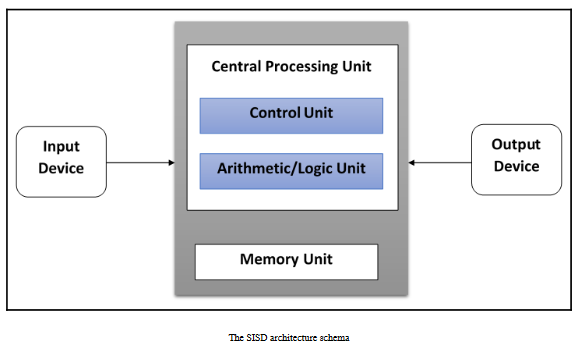
\includegraphics[width=4cm]{figures/kelompok2/chapter1/3.png}
	\centering
	\caption{Algoritma SISD.}
\end{figure}

\noindent
Diagram berikut secara khusus menunjukkan area mana dari CPU yang digunakan pada tahap pengambilan, dekode, dan eksekusi:

\begin{figure}[H]
	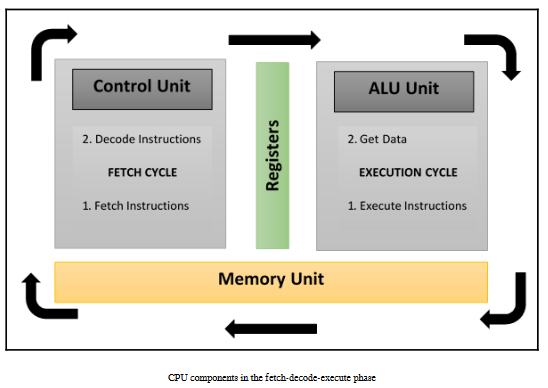
\includegraphics[width=4cm]{figures/kelompok2/chapter1/4.png}
	\centering
	\caption{Area Fetch CPU.}
\end{figure}

\subsection{MISD}
\textit{Multiple Instruction Single Data} \textbf{(MISD)}. Dalam model ini, prosesor, masing-masing dengan unit kontrol mereka sendiri, berbagi unit memori tunggal. Dalam setiap siklus clock, data yang diterima dari memori diproses oleh semua prosesor secara bersamaan, masing-masing sesuai dengan instruksi yang diterima dari unit kontrol. Dalam hal ini, paralelisme (paralelisme tingkat instruksi) diperoleh dengan melakukan beberapa operasi pada bagian data yang sama. Jenis masalah yang dapat dipecahkan secara efisien dalam arsitektur ini agak istimewa, seperti enkripsi data. Untuk alasan ini, komputer MISD belum menemukan ruang di sektor komersial. Komputer MISD lebih dari satu latihan intelektual daripada konfigurasi praktis

\subsection{SIMD}
\textit{Single Instruction Multiple Data} \textbf{(SIMD)}. Sebuah SIMD komputer terdiri dari n prosesor yang identik, masing-masing dengan memori lokal mereka sendiri, di mana dimungkinkan untuk menyimpan data. Semua prosesor bekerja di bawah kendali aliran instruksi tunggal. Selain itu, ada n data stream, satu untuk setiap prosesor. Prosesor bekerja secara simultan pada setiap langkah dan menjalankan instruksi yang sama, tetapi pada elemen data yang berbeda. Ini adalah contoh dari data tingkat paralelisme.
SIMD arsitektur jauh lebih fleksibel daripada arsitektur MISD. Banyak masalah yang mencakup berbagai macam aplikasi dapat diselesaikan dengan algoritma paralel pada komputer SIMD. Fitur lain yang menarik adalah bahwa algoritma untuk komputer ini relatif mudah untuk merancang, menganalisis, dan menerapkan. pembatasan adalah bahwa hanya masalah yang dapat dibagi menjadi beberapa submasalah (yang semuanya identik, yang masing-masing kemudian akan diselesaikan secara simultan melalui set instruksi yang sama) dapat diatasi dengan komputer SIMD.
\subsection{MIMD}
\textit{Multiple Instruction Multiple Data} \textbf{MIMD}. kelas ini merupakan kelas umum dan paling kuat, menurut klasifikasi Flynn. Ini mengandung prosesor, instruksi stream, dan data stream. Setiap prosesor memiliki satuan sendiri kontrol dan memori lokal, yang membuat MIMD arsitektur lebih komputasi kuat dari arsitektur SIMD.
Setiap prosesor beroperasi di bawah kendali aliran instruksi yang dikeluarkan oleh unit kontrol sendiri. Oleh karena itu, prosesor berpotensi dapat menjalankan program yang berbeda dengan data yang berbeda, yang memungkinkan mereka untuk memecahkan submasalah yang berbeda dan dapat menjadi bagian dari masalah yang lebih besar tunggal. Dalam MIMD, arsitektur dicapai dengan bantuan tingkat paralelisme dengan benang dan / atau proses. Ini juga berarti bahwa prosesor biasanya beroperasi asynchronous.

Saat ini, arsitektur ini diterapkan untuk banyak PC, superkomputer, dan jaringan komputer. Namun, ada counter yang perlu Anda pertimbangkan: algoritma asynchronous sulit untuk merancang, menganalisis, dan menerapkan:

\begin{figure}[H]
	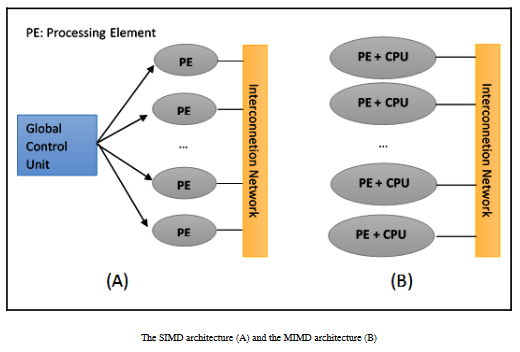
\includegraphics[width=4cm]{figures/kelompok2/chapter1/5.png}
	\centering
	\caption{MIMD.}
\end{figure}

\section{Organisasi Memori}
Aspek lain yang perlu kita pertimbangkan dalam rangka untuk mengevaluasi arsitektur paralel organisasi memori, atau lebih tepatnya, cara di mana data yang diakses. Tidak peduli seberapa cepat unit pengolahan, jika memori tidak dapat mempertahankan dan memberikan petunjuk dan data pada kecepatan yang cukup, maka tidak akan ada peningkatan kinerja. Masalah utama yang kita butuhkan untuk mengatasi untuk membuat waktu respon dari memori yang kompatibel dengan kecepatan prosesor adalah memori waktu siklus, yang didefinisikan sebagai waktu yang telah berlalu antara dua operasi berturut-turut. Waktu siklus prosesor biasanya lebih singkat daripada waktu siklus memori.

Ketika prosesor memulai transfer ke atau dari memori, sumber daya prosesor akan tetap diduduki untuk seluruh durasi siklus memori; Selanjutnya, selama periode ini, tidak ada perangkat lain (misalnya, I / O controller, prosesor, atau bahkan prosesor yang membuat permintaan) akan dapat menggunakan memori karena transfer berlangsung:
\begin{figure}[H]
	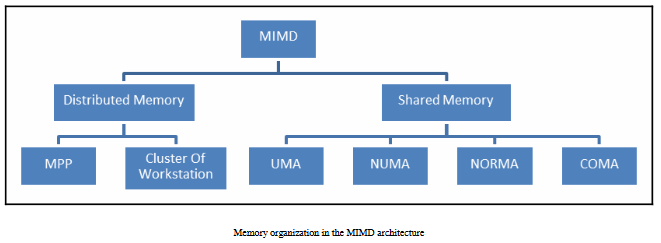
\includegraphics[width=4cm]{figures/kelompok2/chapter1/6.png}
	\centering
	\caption{Memory Organization.}
\end{figure}

\subsection{Shared Memory}

\begin{figure}[H]
	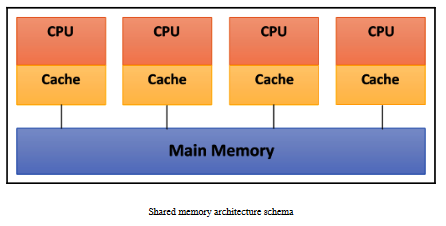
\includegraphics[width=4cm]{figures/kelompok2/chapter1/7.png}
	\centering
	\caption{Shared Memory.}
\end{figure}

\subsection{Distributed Memory}

\begin{figure}[H]
	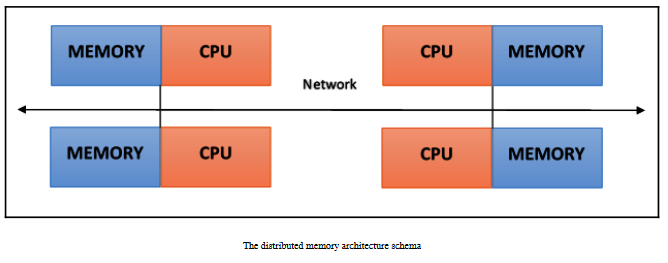
\includegraphics[width=4cm]{figures/kelompok2/chapter1/8.png}
	\centering
	\caption{Distributed Memory.}
\end{figure}

\begin{figure}[H]
	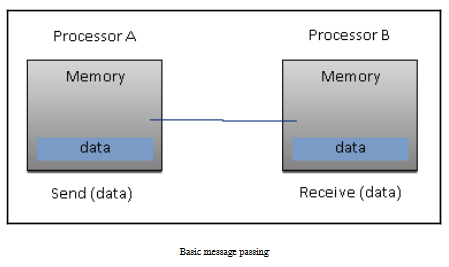
\includegraphics[width=4cm]{figures/kelompok2/chapter1/9.png}
	\centering
	\caption{Distributed Memory 2.}
\end{figure}

\subsection{MPP}

\subsection{Clusters of Workstations}

\subsection{Heterogeneous Architectures}

\begin{figure}[H]
	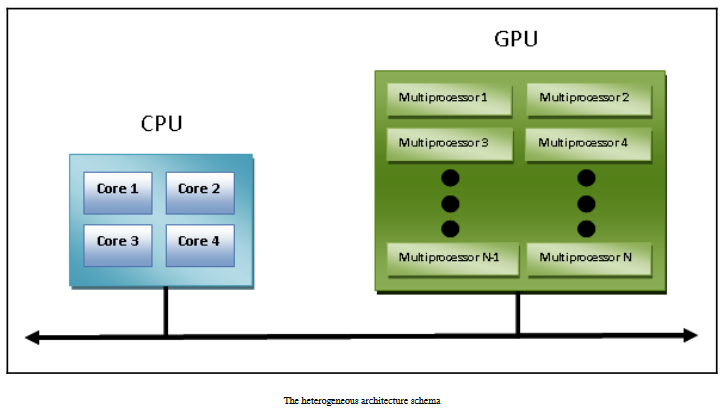
\includegraphics[width=4cm]{figures/kelompok2/chapter1/10.png}
	\centering
	\caption{Architectures.}
\end{figure}